\documentclass[11pt]{article}
\usepackage[utf8]{inputenc}
\usepackage[margin=1in]{geometry}
\usepackage{graphicx}
\usepackage{float}
\usepackage{listings}
\usepackage{xcolor}
\usepackage{hyperref}

\title{Experiment 4: Binary Classification using Linear and Kernel-Based Models}
\author{Monesh M \\ Reg. No: 3122235001084}
\date{February 2026}

\begin{document}

\maketitle

\section{Introduction}
This experiment focuses on binary classification using the Spambase dataset. We compare the performance of Logistic Regression (a linear model) and Support Vector Machines (a kernel-based model). The goal is to accurately classify emails as "Spam" or "Ham" (non-spam).

\section{Exploratory Data Analysis}

\subsection{Class Distribution}
The dataset consists of 4601 instances. The distribution of classes is shown below. We observe a relatively balanced dataset with slightly more non-spam instances.

\begin{figure}[H]
    \centering
    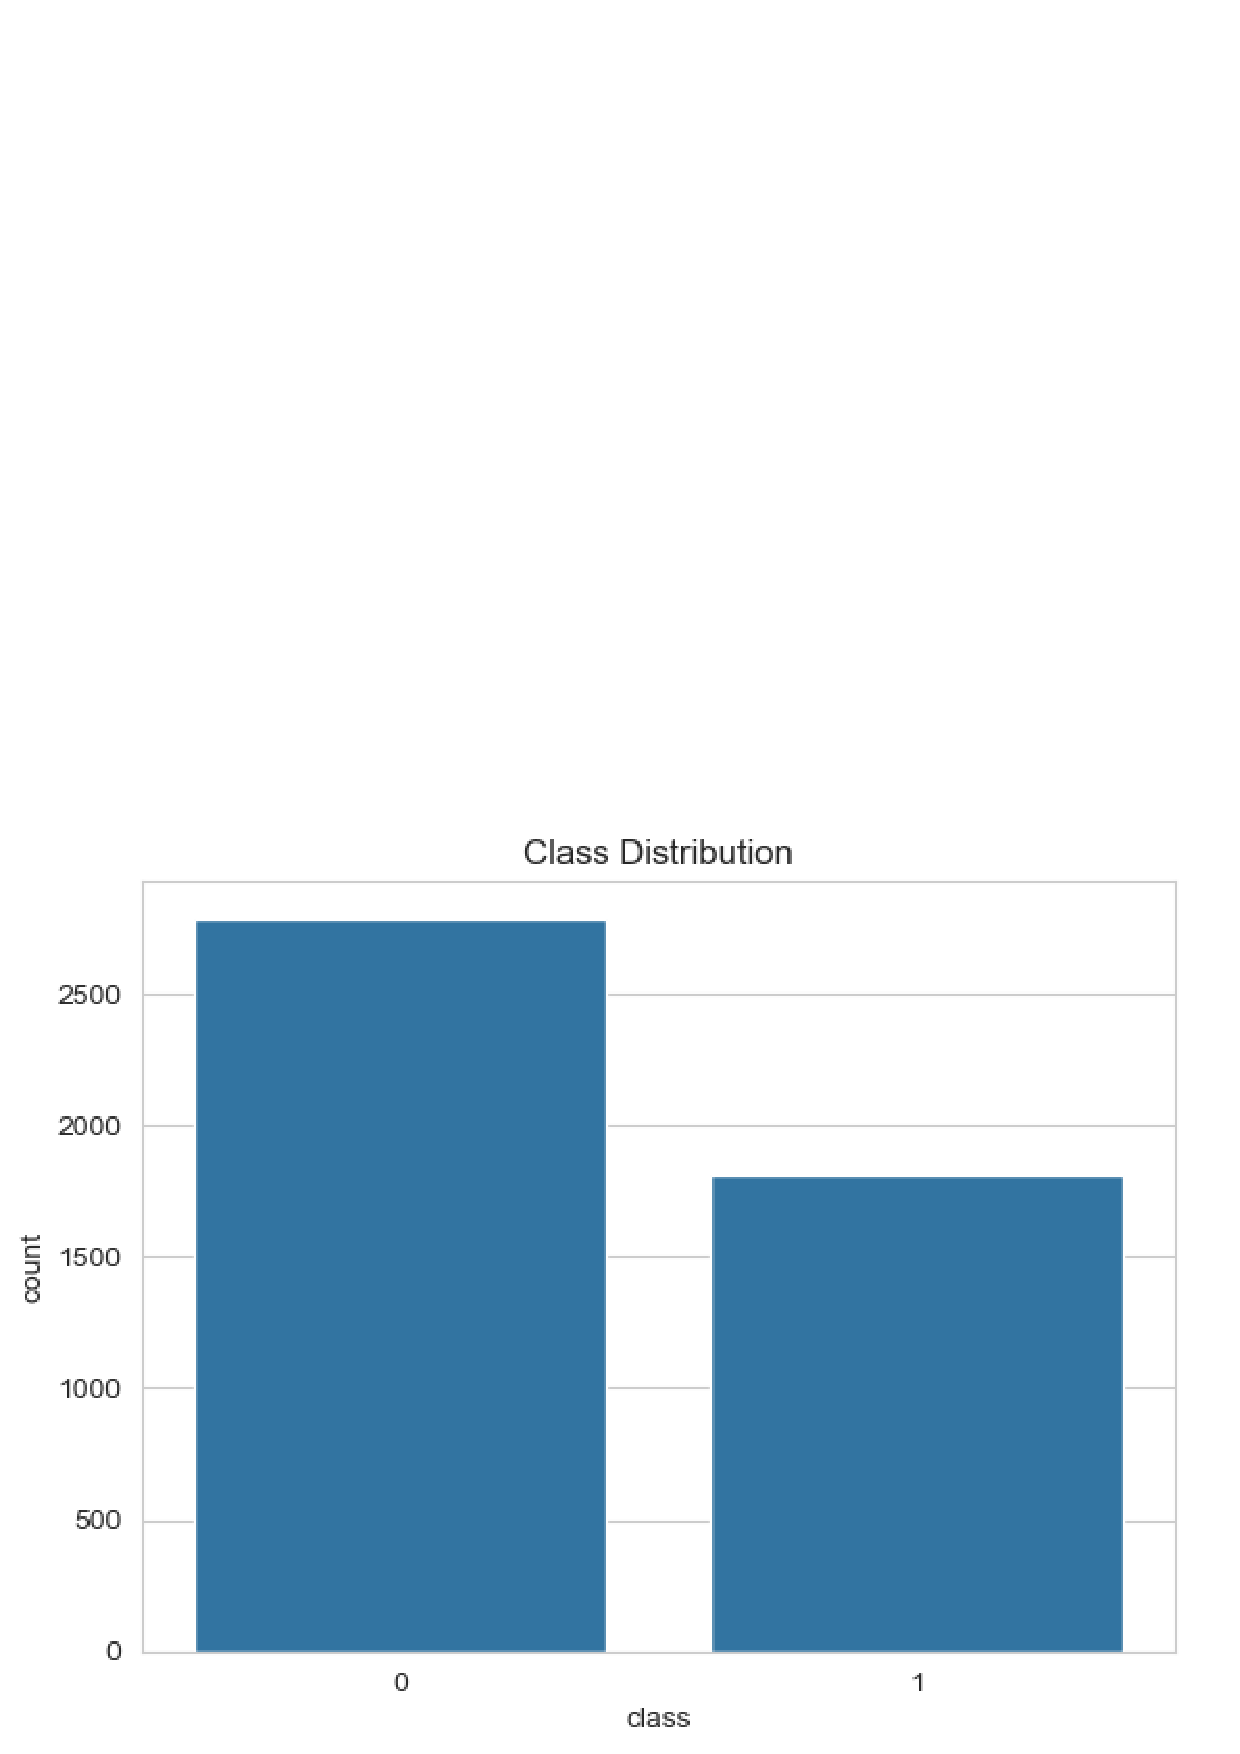
\includegraphics[width=0.6\textwidth]{image/PNG/class_distribution.png}
    \caption{Class Distribution (0: Ham, 1: Spam)}
    \label{fig:class_dist}
\end{figure}

\subsection{Feature Correlation}
The correlation heatmap shows the relationship between different word frequencies and the target class. Some features exhibit strong positive correlations with the spam class.

\begin{figure}[H]
    \centering
    \includegraphics[width=0.8\textwidth]{image/PNG/feature_correlation.png}
    \caption{Feature Correlation Matrix (Top 15 Features)}
    \label{fig:corr}
\end{figure}

\section{Model Implementation}
We used \textbf{Logistic Regression} and \textbf{Support Vector Classification (SVC)}. The data was preprocessed using \texttt{StandardScaler} to normalize the feature ranges.

\section{Performance Evaluation}

\subsection{Confusion Matrices}
Confusion matrices provide a detailed breakdown of correct and incorrect predictions. Both models performed exceptionally well on the test set.

\begin{figure}[H]
    \centering
    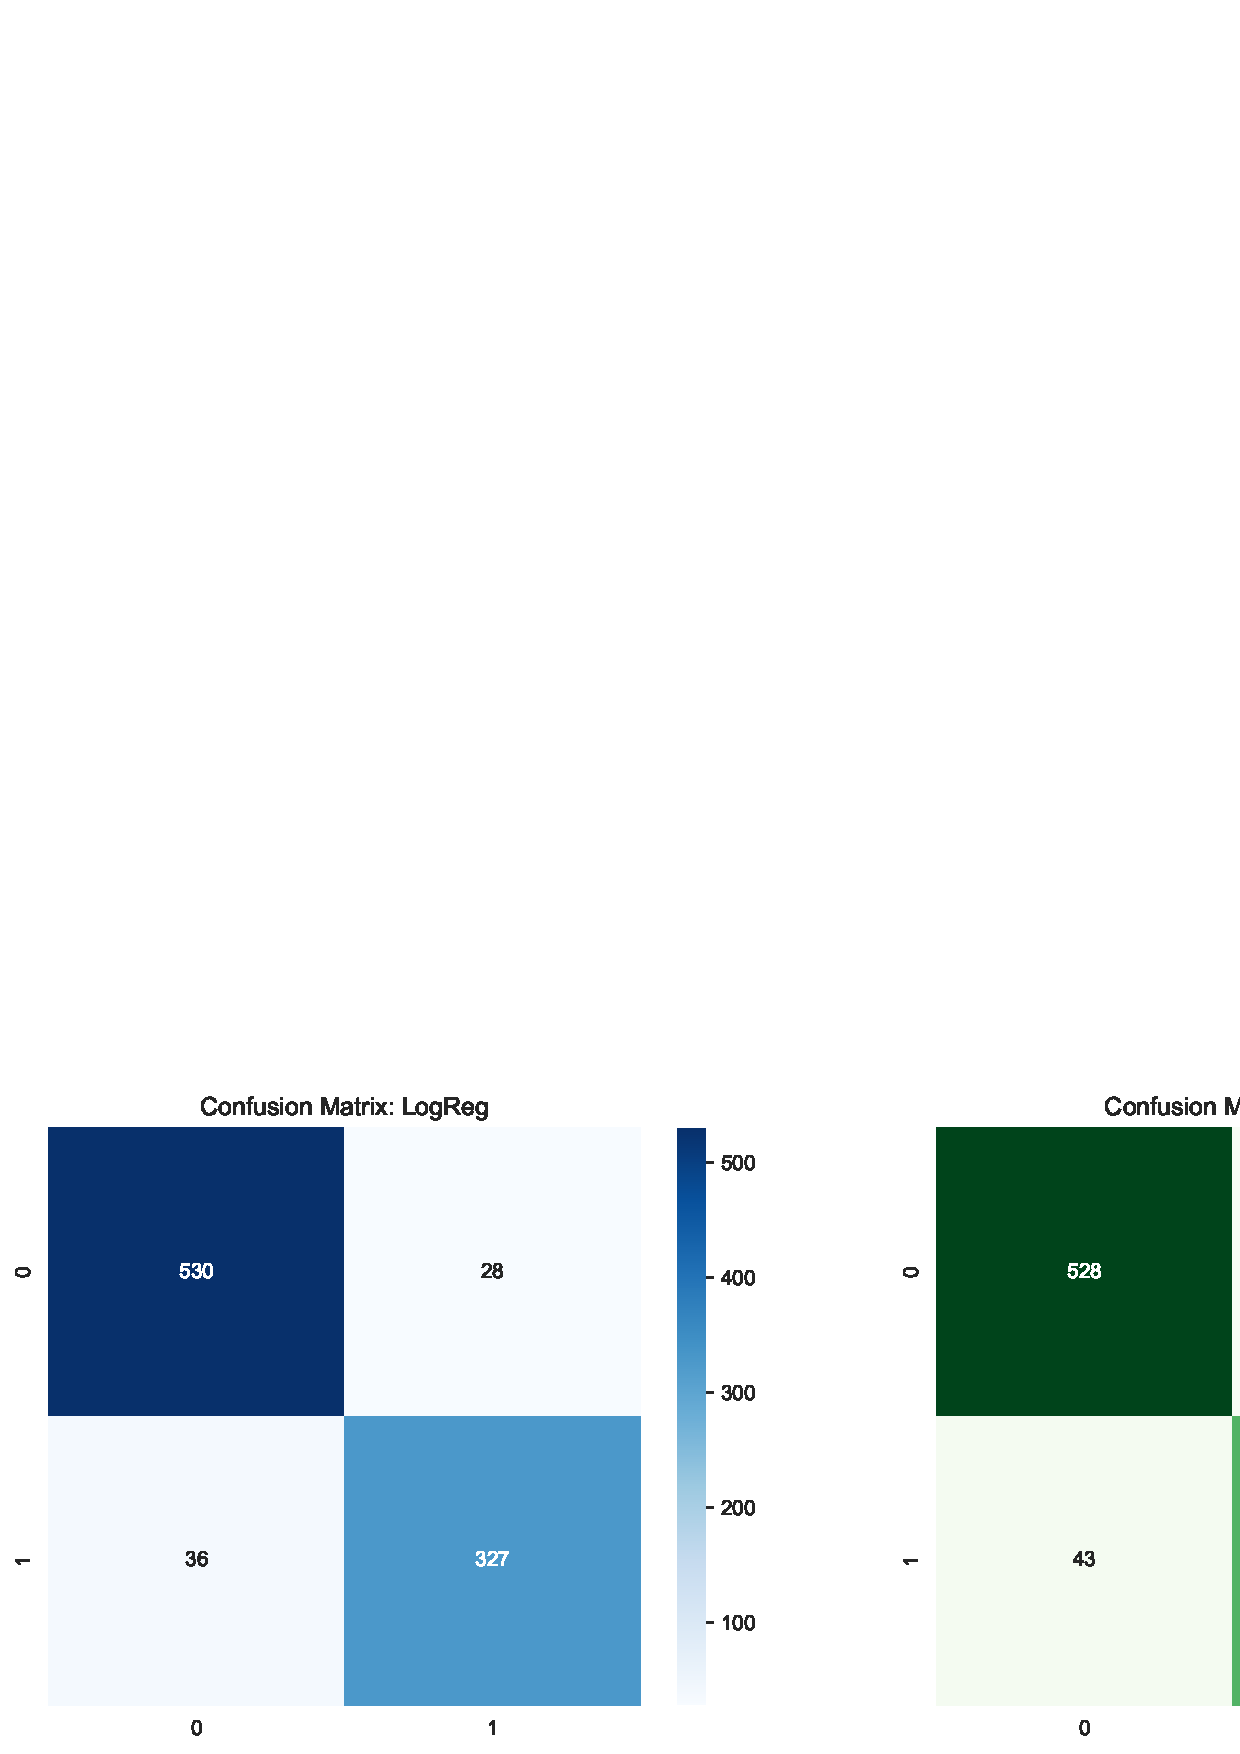
\includegraphics[width=\textwidth]{image/PNG/confusion_matrices.png}
    \caption{Confusion Matrices for LR and SVC}
    \label{fig:cm}
\end{figure}

\subsection{ROC Curves}
The Receiver Operating Characteristic (ROC) curve indicates the diagnostic ability of the classifiers. Both models show high AUC values, indicating strong predictive power.

\begin{figure}[H]
    \centering
    \includegraphics[width=0.7\textwidth]{image/PNG/roc_curve.png}
    \caption{ROC Curve comparison}
    \label{fig:roc}
\end{figure}

\subsection{Learning Curves}
Learning curves help identify if the model is suffering from high bias or high variance. The curves show that both models benefit from increasing training data and stabilize at high accuracy.

\begin{figure}[H]
    \centering
    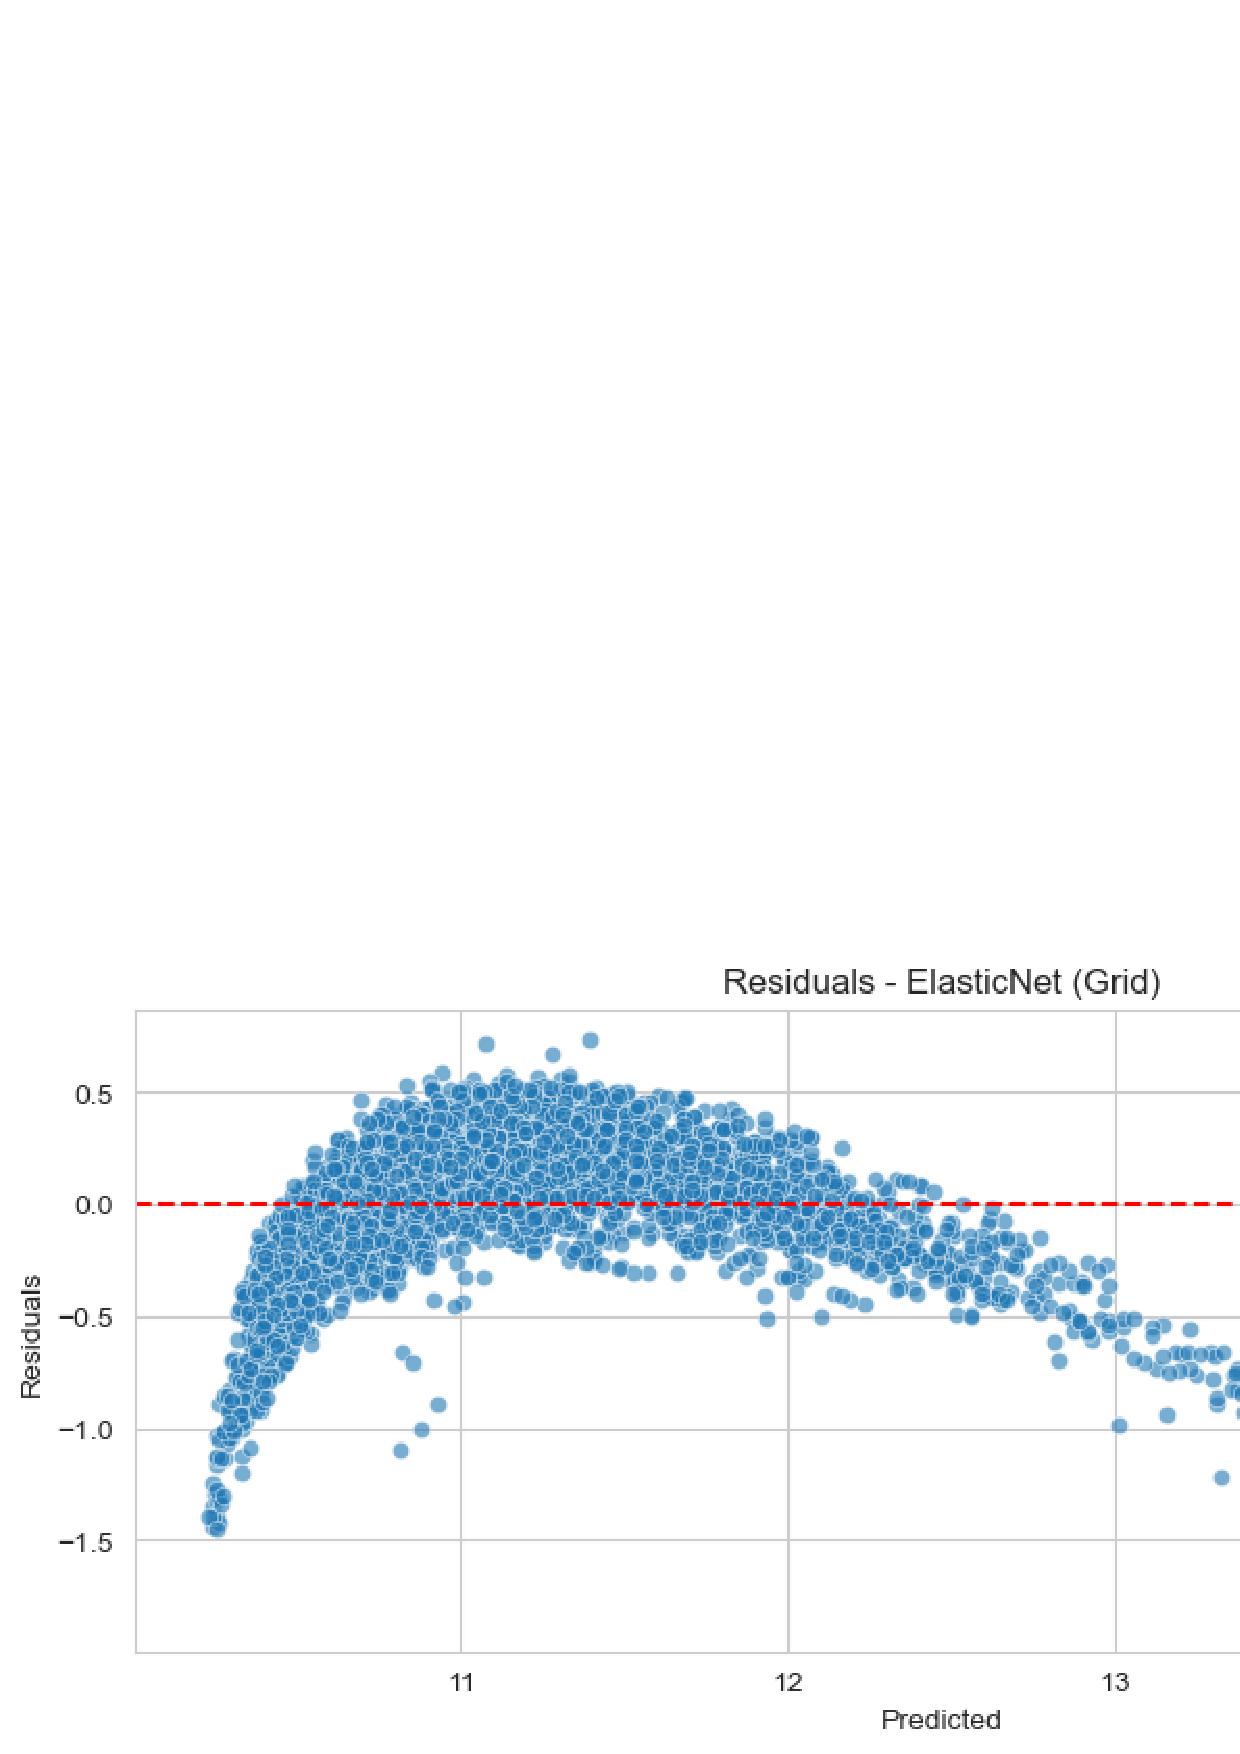
\includegraphics[width=0.7\textwidth]{image/PNG/learning_curves.png}
    \caption{Learning Curves Comparison}
    \label{fig:learning}
\end{figure}

\section{Conclusion}
The experiment successfully demonstrates the application of binary classification models. SVM with RBF kernel and Logistic Regression both achieved accuracy levels above 90\%, emphasizing the effectiveness of character and word frequency features in spam detection.

\end{document}
